%% Ejemplo de la plantilla de latex para las diapositivas del Máster en IA 

%%%%%%%%%%%%%%%%%%%%%%%%%%%%
%% Valores para el ratio de aspecto: 43, 169 
%\documentclass[10pt, envcountsect, presentation, aspectratio=1610, hyperref={hypertexnames=true}]{beamer}
\documentclass[10pt, envcountsect, handout, aspectratio=1610, hyperref={hypertexnames=true}]{beamer}

%%%%%%%%%%%%%%%%%%%%%%%%%%%%

%%%%%%%%%%%%%%%%%%%%%%%%%%%%
%% Incluir fichero de estilo del máster
\input ../style/plantillaMasterIA.sty
%%%%%%%%%%%%%%%%%%%%%%%%%%%%

\addbibresource{../references.bib}



%\setbeameroption{show only notes} % Only notes
%\setbeameroption{show notes on second screen=right}  % Both
%\setbeamertemplate{note page}[compress]
\setbeameroption{hide notes} % Only slides

\renewcommand*\footnoterule{}
\setbeamerfont{footnote}{size=\tiny}




%\input{embed_video.tex}
%\usepackage{movie15}
\usepackage{multimedia}


%%%%%%%%%%%%%%%%%%%%%%%%%%%%
%% Información que aparecerá en la portada
\title[Aprendizaje por Refuerzo]{Aprendizaje por Refuerzo}
\subtitle{Métodos de Monte Carlo} % short title for footer

\author[L. D. Hernández] % Para el pie de página, poner los autores abreviados separados por comas.
{%
	\sc{Luis Daniel Hernández Molinero }\\ % Autor 1
	\textit{Ciencia de la Computación e Inteligencia Artificial}\\  % Area de conocimiento
	\textit{Dept. Ingeniería de la Información y las Comunicaciones}\\  % Departamento
	\\   % No dejes espacio entre esta línea y la llave siguiente 
}

\institute[DIIC]% % Poner las iniciales de los diferentes departamentos de los autores separadas por comas.
{
	\textit{Universidad de Murcia}
}

\newcounter{lastyear}
\setcounter{lastyear}{\the\year}
\addtocounter{lastyear}{-1}

\date{\arabic{lastyear} / \the\year} % Curso académico

%%%%%%%%%%%%%%%%%%%%%%%%%%%%%%%%%%
%% Contenido de las diapositivas
\setbeamerfont{normal text}{size=\normalsize} % Modifica el tamaño del texto de las diapositivas.
\AtBeginDocument{\usebeamerfont{normal text}}

%%%%%%%%%%%%%%%%%%%%%%%%%%%%%%%%%%

\begin{document}	

%%%%%%%%%%%%%%%%%%%%%%%%%%%%%%%%%%









%%%%%%%%%%%%%%%%%%%%%%%%%%%%%%%%%%

\begin{frame}[plain]
	\titlepage
\end{frame}

%%%%%%%%%%%%%%%%%%%%%%%%%%%%%%%%%%

\begin{frame}{Índice de Contenidos}
	\tableofcontents 
	

\end{frame}







%%%%%%%%%%%%%%%%%%%%%%%%%%%%%%%%%%
%%%%%%%%%%%%%%%%%%%%%%%%%%%%%%%%%%
\section{Introducción}

%%%%%%%%%%%%%%%%%%%%%%%%%%%%%%%%%%
%%%%%%%%%%%%%%%%%%%%%%%%%%%%%%%%%%

\begin{frame}{Introducción}
\scalebox{1.3}{
\begin{minipage}{.7\textwidth}
	\begin{itemize}
	\item \key{Programación Dinámica} requiere el conocimiento completo del proceso.
	
	\item Los \key{métodos de Monte Carlo} se caracterizan por:
	\begin{itemize}
		\item Es \key{\textit{sin modelo}}: no requieren conocimiento previo de la dinámica del entorno
		\item Requieren solo \key{experiencia}: conocimiento de trayectorias
		\item Cualquier Monte Carlo usa \key{muestras} para realizar estimaciones.
		\item Una muestra es finita: MC únicamente para \key{tareas episódicas}
		\item \key{Solo al  completar un episodio}, se estimarán los valores y se actualizan las políticas.
		\begin{itemize}
			\item No utiliza \textit{bootstrapping}.
		\end{itemize}
	\end{itemize}
	
	
	\item \key{Métodos de aprendizaje:}
	
	\begin{itemize}
		\item \textbf{Métodos on-policy:} Evalúan o mejoran la política que se utiliza para tomar decisiones.

		\item \textbf{Métodos off-policy:} Evalúan o mejoran una política diferente a la que se utiliza para generar los datos.
	\end{itemize}
	

	
\end{itemize}

\end{minipage}
}


\end{frame}



%%%%%%%%%%%%%%%%%%%%%%%%%%%%%%%%%%%%%%%%%%%%%%%%%%%%%%%%%%%%%%%%%%%%
%%%%%%%%%%%%%%%%%%%%%%%%%%%%%%%%%%%%%%%%%%%%%%%%%%%%%%%%%%%%%%%%%%%%

\section{Métodos On-Policy}



%%%%%%%%%%%%%%%%%%%%%%%%%%%%%%%%%%%%%%%%%%%%%%%%%%%%%%%%%%%%%%%%%%%%
%%%%%%%%%%%%%%%%%%%%%%%%%%%%%%%%%%%%%%%%%%%%%%%%%%%%%%%%%%%%%%%%%%%%

\subsection{Predicción On-policy MC}




%%%%%%%%%%%%%%%%%%%%%%%%%%%%%%%%%%%%%%%%%%%%%%%%%%%%%%%%%%%%%%%%%%%%
%%%%%%%%%%%%%%%%%%%%%%%%%%%%%%%%%%%%%%%%%%%%%%%%%%%%%%%%%%%%%%%%%%%%

\subsubsection{Evaluación de las funciones $v(s)$}


%%%%%%%%%%%%%%%%%%%%%%%%%%%%%%%%%%
%%%%%%%%%%%%%%%%%%%%%%%%%%%%%%%%%%
\begin{frame}{Evaluación de Políticas Monte-Carlo (On-Policy)}
	
	\begin{itemize}
		\item Para \key{predicción}:  
			\begin{itemize}
				\item Entrada: MDP $\langle S,A,P,R, \gamma \rangle$ y política $\pi$.
				\item Salida, función de valor $v_\pi$.
			\end{itemize}
		
		\item En  \key{Programación Dinámica:} :  $V(s) \gets \sum_{a} \pi(a|s) \sum_{s', r} {\color{red}p(s', r | s, a)} [r + \gamma V(s')]$ (utiliza \textit{bootstrapping})
		
		\item Pero \key{también sabemos} que:
		
		\begin{itemize}
			\item\textbf{ Por definición}, $\ds v_\pi(s) = \mathbb{E}_\pi \left[ G_t| s_t=s \right]$ con $	G_t = R_{t+1} + \gamma R_{t+2} + \gamma^2 R_{t+3} + \dots $ (\key{variable aleatoria}).
		
		\item \textbf{Ley de los grandes números}, $\ds\mathbb{E}_\pi[G_t|s_t=s] \approx  \frac{1}{N} \sum_{i=1}^{N} G_t^{(i)}$. \hfill$ {\displaystyle \operatorname {P} \left(\lim _{n\rightarrow \infty }{\overline {X}}_{n}=\mu \right)=1,}$ 
			
		\end{itemize}

	

			\item \key{Objetivo MC}: Aprender $v_\pi$ a partir de episodios de experiencia bajo la política $\pi$.
				\begin{enumerate}
					\item Soltar al agente en $S_0$.
					\item Obtener un episodio: $S_0, A_1, R_1, \ldots, S_T, R_T \sim \pi$.
					\item Calcular su retorno: $G_0 = R_{1} + \gamma R_{2} + \ldots + \gamma^{T-1}R_T$
					\item Repetir varias veces los 3 pasos anteriores.
					\item Retornar el promedio de los retornos.
				\end{enumerate}
				
			\centerline{$S_0, \underbrace{S_1, R_1, \overbrace{S_2,R_2,\underbrace{S_3,R_3\ldots, S_T, R_T}_{G_3}}^{G_1}}_{G_0}$ \qquad Usamos el Proceso de Recompensas de Markov}

	\end{itemize}
\end{frame}




%%%%%%%%%%%%%%%%%%%%%%%%%%%%%%%%%%
%%%%%%%%%%%%%%%%%%%%%%%%%%%%%%%%%%
\begin{frame}{Evaluación de Políticas por Monte-Carlo}{Por Primera visita y por Todas las Visitas}
\begin{itemize}
	\item\key{ Evaluación de Primera Visita (First-Visit)}
		\hfil $S_0,S_1,R_1\ldots, \underbrace{{\color{reddark} S_i},R_i\ldots,{\color{reddark} S_i},R_i\ldots S_T,R_T}_{G_i}$
		
	\begin{itemize}
		\item Para evaluar el estado $s$:
		\begin{itemize}
			\item \key{Identifica el primer instante} de tiempo $t$ en el que el estado $s$ es visitado en un episodio.
			\item Incrementa el contador $N(s) \leftarrow N(s) + 1$.
			\item Incrementa el retorno total $S(s) \leftarrow S(s) + G_t$.
		\end{itemize}
		\item El valor se estima como el retorno promedio: $V(s) = \frac{S(s)}{N(s)}$.
		\item Según la ley de los grandes números, $V(s) \to v_\pi(s)$ a medida que $N(s) \to \infty$.
	\end{itemize}
	
	
	
	\item \key{Evaluación de Todas las Visitas (Every-Visit)}
	\hfil $S_0,S_1,\ldots, \underbrace{{\color{reddark} S_i},R_i\ldots,\overbrace{{\color{reddark} S_i},R_i\ldots S_T,R_T}^{G'_i}}_{G_i}$
	
	
	
	\begin{itemize}
		\item Para evaluar el estado $s$:
		\begin{itemize}
			\item \key{En cada instante} de tiempo $t$ en el que el estado $s$ es visitado en un episodio:

				 $1.$ Incrementa el contador $N(s) \leftarrow N(s) + 1$.
				
				 $2.$ Incrementa el retorno total $S(s) \leftarrow S(s) + G_t$.

		\end{itemize}
		\item El valor se estima como el retorno promedio: $V(s) = \frac{S(s)}{N(s)}$.
		\item Nuevamente, $V(s) \to v_\pi(s)$ a medida que $N(s) \to \infty$.  \citep{singh1996reinforcement}
	\end{itemize}
	
	\item \key{Actualización incremental:} $N(s) \leftarrow N(s) + 1$, $V(s) \leftarrow V(s) + \frac{1}{N(s)}(G_t - V(s))$
\end{itemize}


\end{frame}



%%%%%%%%%%%%%%%%%%%%%%%%%%%%%%%%%%
%%%%%%%%%%%%%%%%%%%%%%%%%%%%%%%%%%



%%%%%%%%%%%%%%%%%%%%%%%%%%%%%%%%%%
%%%%%%%%%%%%%%%%%%%%%%%%%%%%%%%%%%
\begin{frame}{Evaluación de Políticas Monte-Carlo (Predicción)}{\cite{Sutton2018}}
	

\begin{algorithm}[H]
	\caption{Predicción MC de primera visita, para estimar \(V \approx v_\pi\)}
	
	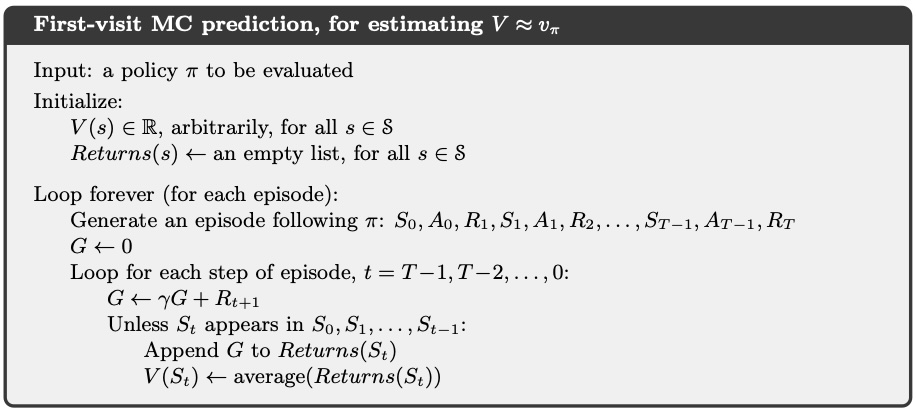
\includegraphics[width=\textwidth]{fig/first-visitMC}
\end{algorithm}

\end{frame}



%%%%%%%%%%%%%%%%%%%%%%%%%%%%%%%%%%
%%%%%%%%%%%%%%%%%%%%%%%%%%%%%%%%%%
\begin{frame}{Resumen. Predicción Monte Carlo}
	\scalebox{1.2}{
		\begin{minipage}{.8\textwidth}
			\begin{itemize}
				\item Los métodos Monte Carlo \key{no usan \textit{bootstraping}}.
				\begin{itemize}
					\item La estimación para un estado no se construye a partir de la estimación de ningún otro estado, 
					como ocurre en la Programación Dinámica (DP).
				\end{itemize} 
				\item El costo computacional de estimar el valor de un solo estado \key{es independiente} del número total de estados.
				\item Los métodos Monte Carlo son particularmente \textbf{atractivos} 
				cuando se requiere el valor de \key{\textit{solo uno o un subconjunto de estados}}.
			\end{itemize}
		\end{minipage}
	}
\end{frame}

%%%%%%%%%%%%%%%%%%%%%%%%%%%%%%%%%%
%%%%%%%%%%%%%%%%%%%%%%%%%%%%%%%%%%
\begin{frame}{Ejemplo de Blackjack}
	
	\begin{itemize}
		\item \textbf{Estados} (200 en total):
		\begin{itemize}
			\item Suma actual (12-21).
			\item Carta visible del dealer (as-10).
			\item ¿Tengo un as "\/utilizable"\/? (sí-no).
		\end{itemize}
		\item \textbf{Acciones}:
		\begin{itemize}
			\item \textit{Pedir}: recibir otra carta (sin reemplazo).
			\item \textit{Plantarse}: detenerse y terminar.
		\end{itemize}
		\item \textbf{Recompensa al plantarse}:
		\begin{itemize}
			\item $+1$ si la suma de cartas del jugador es\\  mayor que la suma de cartas del croupier.
			\item $0$ si las sumas son iguales.
			\item $-1$ si la suma del jugador es \\ menor que la suma del croupier.
		\end{itemize}
		\item \textbf{Recompensa al pedir}:
		\begin{itemize}
			\item $-1$ si la suma de cartas del jugador $> 21$ (termina el juego).
			\item $0$ en caso contrario.
		\end{itemize}
		\item \textbf{Transiciones}: automáticamente pide si la suma de cartas del jugador $< 12$.
		
		\item \textbf{Política:} plantarse si la suma de cartas $\geq 20$, de lo contrario pedir.
	\end{itemize}
	
\TPMargin{0mm}%
\begin{textblock}{11}(7, 3) \small
	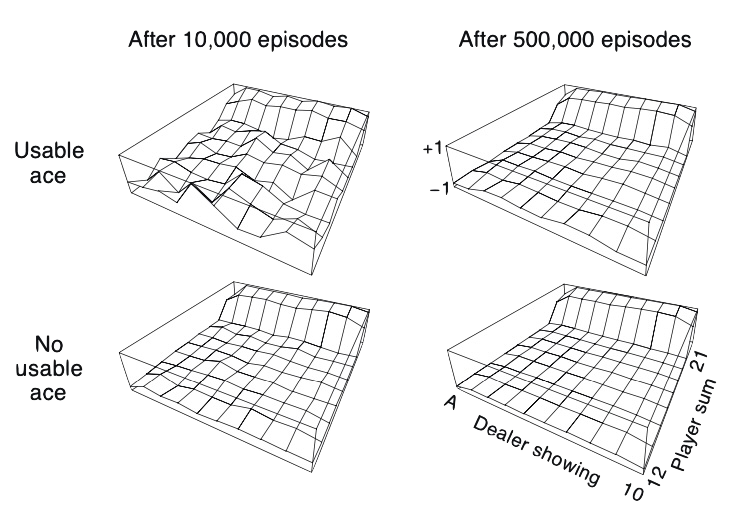
\includegraphics[width=0.8\textwidth]{fig/blackjack_value_function.png}
\end{textblock}


\end{frame}






%%%%%%%%%%%%%%%%%%%%%%%%%%%%%%%%%%%%%%%%%%%%%%%%%%%%%%%%%%%%%%%%%%%%
%%%%%%%%%%%%%%%%%%%%%%%%%%%%%%%%%%%%%%%%%%%%%%%%%%%%%%%%%%%%%%%%%%%%

\subsection{Control On-policy}




%%%%%%%%%%%%%%%%%%%%%%%%%%%%%%%%%%%%%%%%%%%%%%%%%%%%%%%%%%%%%%%%%%%%
%%%%%%%%%%%%%%%%%%%%%%%%%%%%%%%%%%%%%%%%%%%%%%%%%%%%%%%%%%%%%%%%%%%%

\subsubsection{Evaluación de las funciones $q(s,a)$}

%%%%%%%%%%%%%%%%%%%%%%%%%%%%%%%%%%
%%%%%%%%%%%%%%%%%%%%%%%%%%%%%%%%%%
\begin{frame}{Evaluación de Funciones $q()$ (Control)}
	
	\begin{itemize}
		\item Para \key{control}:  
		\begin{itemize}
			\item Entrada: MDP $\langle S,A,P,R, \gamma \rangle$.  
			\item Salida: función de valor óptima $v^*(s)$ y política óptima $\pi^*(s)$
			
		\end{itemize}
		
		\item Para  \key{Programación Dinámica:}  $\pi'(s) \gets \arg_a\max q_\pi(s,a) = \arg\max_a \sum_{s', r} {\color{red} p(s', r | s, a)} [r + \gamma V(s')]$
		
		\item Pero \key{también sabemos} que:
		
		\begin{itemize}
			\item \textbf{Por definición}, $\ds q_\pi(s,a) = \mathbb{E}_\pi \left[ G_t| s_t=s, a_t=a \right]$ con $	G_t = R_{t+1} + \gamma R_{t+2} + \gamma^2 R_{t+3} + \dots $.
			
			\item\textbf{ Ley de los grandes números:} $\ds\mathbb{E}_\pi[G_t|s_t=s, a_t=a] \approx  \frac{1}{N} \sum_{i=1}^{N} G_t^{(i)}$. \hfill$ {\displaystyle \operatorname {P} \left(\lim _{n\rightarrow \infty }{\overline {X}}_{n}=\mu \right)=1,}$ 
		\end{itemize}
		
		
		
		
		\item \key{Objetivo MC}: Aprender $q_\pi$ a partir de episodios de experiencia bajo la política $\pi$.
		
		\item Ahora en vez de tener en cuenta el estado, hay que tener en cuenta (estado, acción)
		
		\centerline{\footnotesize $\underline{S_0, A_0}, \underbrace{R_1, \underline{S_1, A_1} \ldots \underline{S_i,A_i}, \overbrace{R_{i+1},{S_{i+1},\ldots, R_T, S_T}}^{G_i(S_i, A_i)}}_{G_0 (S_0, A_0)}$}
		
		\item Se visita un par estado–acción \((s, a)\) en un episodio si el estado \(s\) se visita y la acción \(a\) se toma en él.
		
		\item El método MC de \key{todas las visitas} estima el valor de un par estado–acción como el promedio de los retornos que siguieron a todas las visitas a este. 
		\item El método MC de \key{primera visita} promedia los retornos que siguieron a la primera vez en cada episodio en que el estado fue visitado y la acción seleccionada. 
		\item Ambos  convergen  a los valores esperados verdaderos.
	\end{itemize}
	
\end{frame}





%%%%%%%%%%%%%%%%%%%%%%%%%%%%%%%%%%
%%%%%%%%%%%%%%%%%%%%%%%%%%%%%%%%%%
\begin{frame}{Hay problemas}
	\scalebox{1.3}{
		\begin{minipage}{1.2\textwidth}
			\begin{itemize}
				
				\item Se tiene un \key{problema de exploración} (como en bandido k-brazos)
				
				P.e. Si \(\pi\) es una \textbf{política determinista}
				\begin{itemize}
					\item Algunos pares estado-acción pueden no ser visitados nunca.
					\item Así es imposible saber si hay alternativas posibles.
				\end{itemize}
				
				~
				
				~
				
				\item \key{Soluciones:}
				\begin{itemize}
					\item \textbf{Inicios exploratorios:} $s_0 \sim rnd(\c{S})$ y $a_0\sim rnd(\c{A}(s_0))$
					\item \textbf{Políticas estocásticas:} $\pi(s|a)>0$ \quad $\forall s \in \c{S}, \forall a\in \c{A}$
				\end{itemize}
			\end{itemize}
		\end{minipage}
	}	
\end{frame}






%%%%%%%%%%%%%%%%%%%%%%%%%%%%%%%%%%
%%%%%%%%%%%%%%%%%%%%%%%%%%%%%%%%%% 
\subsubsection{Iteración General de  Políticas para MC}

%%%%%%%%%%%%%%%%%%%%%%%%%%%%%%%%%%
%%%%%%%%%%%%%%%%%%%%%%%%%%%%%%%%%% 
\begin{frame}{Iteración  de  Políticas General}
	
	
	\centerline{\raisebox{0.25cm}{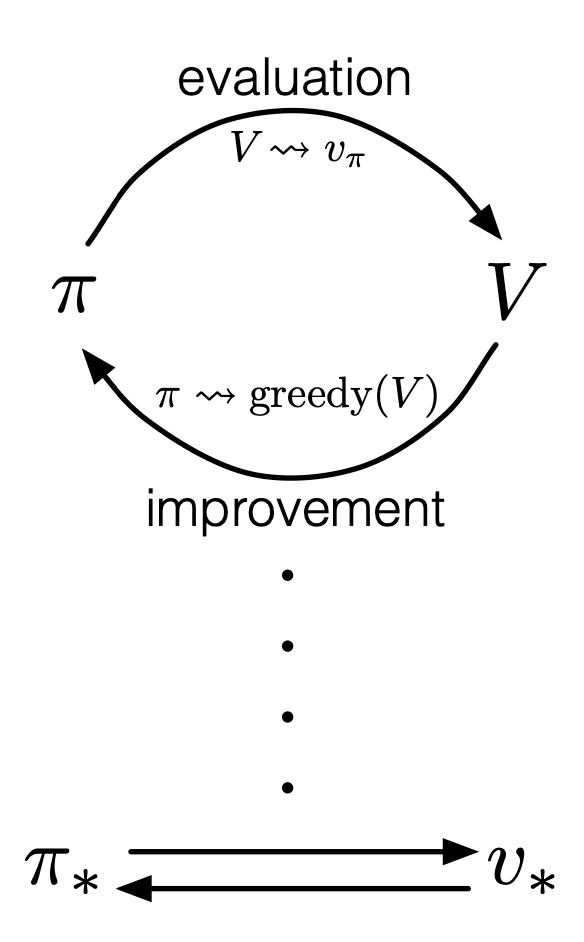
\includegraphics[width=.20\textwidth, trim=0 200 0 0, clip]{fig/iteracion_generalizada}} \hspace{2cm}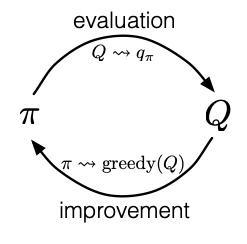
\includegraphics[width=0.20\textwidth]{fig/MejoraPolitica}}
	
	\vfill
	
	\begin{itemize}
		\item La idea general de la \key{Iteración de Políticas}:
		
		\centerline{$\pi_0 \stackrel{E}{\longrightarrow} v_{\pi_0} \stackrel{I}{\longrightarrow} \pi_1 \stackrel{E}{\longrightarrow} v_{\pi_1} \stackrel{I}{\longrightarrow} \pi_2 \stackrel{E}{\longrightarrow} \dots \stackrel{I}{\longrightarrow} \pi_* \stackrel{E}{\longrightarrow} v_*$}
		
		\item \key{Versión Monte Carlo} de la iteración clásica de políticas. 
		
		\centerline{$
			\pi_0 \overset{\text{E}}{\longrightarrow} q_{\pi_0} \overset{\text{I}}{\longrightarrow} \pi_1 \overset{\text{E}}{\longrightarrow} q_{\pi_1} \overset{\text{I}}{\longrightarrow} \pi_2 \overset{\text{E}}{\longrightarrow} \cdots \overset{\text{I}}{\longrightarrow} \pi_* \overset{\text{E}}{\longrightarrow} q_*
			$}
		
		\begin{itemize}
			\item \key{Evaluación:} Simulación por muestras de cada $q_{\pi_k}(s, a)$
			\item\key{ Mejora}: $\pi_{k+1}(s) = \arg\max_a q_{\pi_k}(s, a)$
			
			\item \key{Hipótesis:} un número infinito de episodios + los episodios \textit{se generan con inicios exploratorios}.
			\begin{itemize}
				\item los métodos de Monte Carlo calcularán cada $q_{\pi_k}$ exactamente, para $\pi_k$ arbitrarias.
				\item Se sigue cumpliento el teorema de mejora de políticas
				
				Como $q_{\pi_k}(s, \pi_{k+1}(s)) \geq v_{\pi_k}(s)$, entonces $v_{\pi_{k+1}}(s)\geq v_{\pi_k}(s)$  ($\pi_{k+1}$ es tan buena como $\pi_k$)
			\end{itemize}
			
			\item \key{En la práctica} renunciamos al número infinito de episodios (Renunciamos a una evaluación exacta).
			
			\centerline{$
			\pi_0 \overset{\text{E}}{\longrightarrow} Q_{\pi_0} \overset{\text{I}}{\longrightarrow} \pi_1 \overset{\text{E}}{\longrightarrow} Q_{\pi_1} \overset{\text{I}}{\longrightarrow} \pi_2 \overset{\text{E}}{\longrightarrow} \cdots \overset{\text{I}}{\longrightarrow} \pi_* \overset{\text{E}}{\longrightarrow} q_*
			$}
			
			
			
		\end{itemize}
		
		%	\item Estretegias:
		%		\begin{itemize}
			%			\item On-policy. Usando la política
			%			\item Off-policy. Fuera de la política
			%		\end{itemize}
		%		
		
	\end{itemize}
	
\end{frame}








%%%%%%%%%%%%%%%%%%%%%%%%%%%%%%%%%%
%%%%%%%%%%%%%%%%%%%%%%%%%%%%%%%%%% 
\subsubsection{Con inicios exploratorios}

%%%%%%%%%%%%%%%%%%%%%%%%%%%%%%%%%%
%%%%%%%%%%%%%%%%%%%%%%%%%%%%%%%%%%
\begin{frame}{Iteración de Valor versión Monte Carlo con Inicios Exploratorios}{\cite{Sutton2018}}
	
	\begin{algorithm}[H]
		\caption{Monte Carlo ES (Exploring Starts), para estimar \(\pi \approx \pi_*\)}
		
		\centering 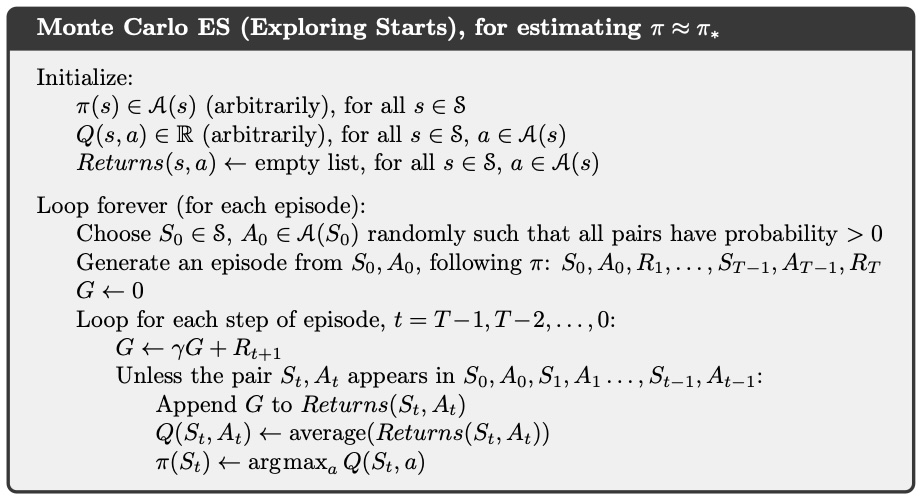
\includegraphics[width=.88\textwidth]{fig/MC-ES}
	\end{algorithm}
	
	\TPMargin{0mm}%
	\begin{textblock}{4.3}(10.1, 5.2) \small
		\begin{tcolorbox}[colback=blue!5!white]\footnotesize
			\hspace{-0.9cm} \faCaretSquareRight ~	\hbox{Los returns se acumulan} \textbf{independientemente} de la política que los observó.
			
			\hspace{-0.4cm} \faCaretSquareRight	~ No converge a una política subóptima
		\end{tcolorbox}
	\end{textblock}

\end{frame}




%%%%%%%%%%%%%%%%%%%%%%%%%%%%%%%%%%
%%%%%%%%%%%%%%%%%%%%%%%%%%%%%%%%%%
\begin{frame}{Resolver el Blackjack por MC}
	
	\begin{columns}
		\scalebox{1.1}{	\begin{column}{.6\textwidth}
				\begin{itemize}
					\item Queremos resolver Blackjack por MC-ES
					\item Para garantizar la exploración completa:
					\begin{itemize}
						\item Se seleccionan al azar las cartas del crupier.
						\item Se elige la suma inicial del jugador.
						\item Se determina si el jugador tiene o no un as utilizable.
						\item Todas las combinaciones posibles se generan con igual probabilidad.
					\end{itemize}
					\item Política inicial: Se planta solo con sumas de 20 o 21, de lo contrario pedir.
					\item Los valores iniciales de la función de valor de acción (\(Q(s, a)\)) se establecen en cero para todos los pares estado-acción.
					%			\item La política óptima encontrada mediante Monte Carlo ES coincide con la estrategia "básica" de Thorp (1966), con una excepción:
					%			\begin{itemize}
						%				\item Una muesca en la política para un as utilizable, no presente en la estrategia de Thorp.
						%			\end{itemize}
					%			\item La discrepancia mencionada no tiene explicación conocida, pero se confía en que la política obtenida es óptima para la versión del blackjack descrita.
					\item 	El jugador aplica una política diferente dependiendo de si tiene o no un as utilizable.
				\end{itemize}
		\end{column}}		
		\begin{column}{.4\textwidth}
			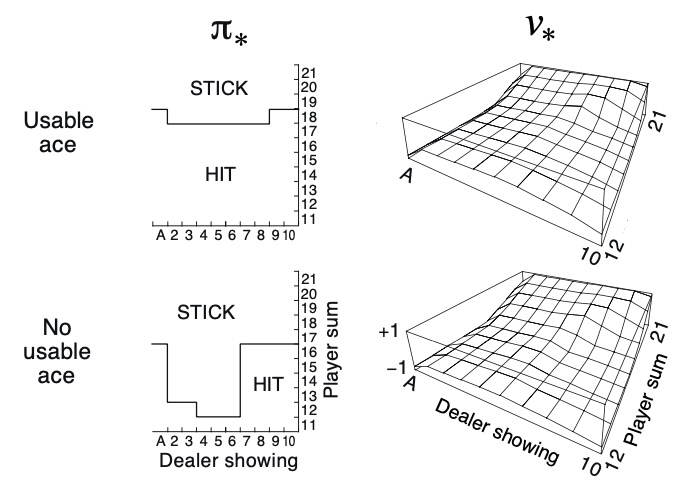
\includegraphics[width=\textwidth]{fig/blackjack_policy}		
		\end{column}		
	\end{columns}
	

\end{frame}




%%%%%%%%%%%%%%%%%%%%%%%%%%%%%%%%%%
%%%%%%%%%%%%%%%%%%%%%%%%%%%%%%%%%% 
\subsubsection{Con políticas $\epsilon$-soft}


%%%%%%%%%%%%%%%%%%%%%%%%%%%%%%%%%%
%%%%%%%%%%%%%%%%%%%%%%%%%%%%%%%%%%
\begin{frame}{Iteración de Valor versión Monte Carlo con Soft-Policy}{\cite{Sutton2018}}
	
	
	\begin{itemize}
		\item \key{Recuerda}. Las soluciones para garantizar que sean seleccionados los pares (estado, acción):
		\begin{itemize}
			\item \textbf{Inicios exploratorios:} $s_0 \sim rnd(\c{S})$ y $a_0\sim rnd(\c{A}(s_0))$
			\item \textbf{Políticas estocásticas:} $\pi(s|a)>0$ \quad $\forall s \in \c{S}, \forall a\in \c{A}$
		\end{itemize}
		
		\item \key{Política suave (soft-policy):} \(\pi(a|s) > 0\) para todos los \(s \in \mathcal{S}\) y \(a \in \mathcal{A}\).
		
		\item \key{Política \(\color{blue} \epsilon\)-soft:} \(\ds \pi(a|s) \geq \frac{\epsilon}{|\mathcal{A}(s)|}\) para todos los \(s \in \mathcal{S}\) y \(a \in \mathcal{A}\), donde \(\epsilon > 0\).
		
		
		
		
		La acción codiciosa (greedy) se selecciona con probabilidad:
		$\ds
		1 - \epsilon + \frac{\epsilon}{|\mathcal{A}(s)|}
		$
		mientras que una acción no codiciosa específica se selecciona con probabilidad:
		$\ds
		\frac{\epsilon}{|\mathcal{A}(s)|}.
		$
		
		\begin{itemize}
			\item \key{Las políticas \(\epsilon\)-\textbf{greedy} son políticas \textbf{$\epsilon$-\textit{soft}}}
			
			\hfil $a^* \gets
			\begin{cases}
				\arg\max_a Q_\pi(s,a) & \text{\color{black} con probabilidad } 1 - \epsilon + \frac{\epsilon}{|\mathcal{A}(s)|} \mbox{\hspace{1cm}\color{black}  (rompiendo aleatoriamente)} \\
				\text{acción no greedy} & \text{\color{black} con probabilidad }  \frac{\epsilon}{|\mathcal{A}(s)|}
			\end{cases}$
			
		\end{itemize}
		
		
		
		
		\item \key{Generalized Policy Iteration (GPI):} No requiere que la política se lleve completamente a una política-greedy, solo que se mueva en dirección hacia una política-greedy, de forma análoga a que tampoco evaluamos completamente las funciones de valor.
	\end{itemize}
	

\end{frame}






%%%%%%%%%%%%%%%%%%%%%%%%%%%%%%%%%%
%%%%%%%%%%%%%%%%%%%%%%%%%%%%%%%%%%
\begin{frame}{La Iteración de Políticas Funciona para Políticas Greedy sobre Políticas \(\epsilon\)-soft.}
	
	
	\begin{itemize}
		\item {Cualquier política} $\pi'$ que sea \(\epsilon\)-\textit{\color{blue}greedy} con respecto a \(q_\pi\) \textit{\color{blue} es una mejora} sobre cualquier política \(\epsilon\)-\textit{\color{blue} soft}, \(\pi\), 
		
		\begin{itemize}
			\item Se cumple que: $q_\pi(s, \pi'(s)) \geq  v_\pi(s)$
			
			{\footnotesize
				\begin{align*}
					q_\pi(s, \pi'(s)) &= \sum_a \pi'(a|s) q_\pi(s, a) \notag \\
					&= \frac{\varepsilon}{|\mathcal{A}(s)|} \sum_a q_\pi(s, a) + (1 - \varepsilon) \max_a q_\pi(s, a)  \\
					&\geq \frac{\varepsilon}{|\mathcal{A}(s)|} \sum_a q_\pi(s, a) + (1 - \varepsilon) \sum_a \left(\pi(a|s) - \frac{\varepsilon / |\mathcal{A}(s)|}{1 - \varepsilon}\right) q_\pi(s, a) \notag \\
					&= \frac{\varepsilon}{|\mathcal{A}(s)|} \sum_a q_\pi(s, a) - \frac{\varepsilon}{|\mathcal{A}(s)|} \sum_a q_\pi(s, a) + \sum_a \pi(a|s) q_\pi(s, a) \\
					&= v_\pi(s).
				\end{align*}
			}
			
			\item\textbf{ Por el teorema de mejora de políticas}, \(\pi' \succeq \pi\) (es decir, \(v_{\pi'}(s) \geq v_\pi(s)\) para todo \(s \in S\)).
			
		\end{itemize}
		
		\item $v_{\pi'}(s) = v_{\pi}(s)$ para todo  \(s \in S\) solo cuando \key{tanto \(\pi '\) como \(\pi\) son óptimas entre las políticas \(\epsilon\)-soft}; es decir, cuando son mejores o iguales que todas las demás políticas \(\epsilon\)-soft \citep{Sutton2018}.
		
	\end{itemize}
	

\end{frame}


%%%%%%%%%%%%%%%%%%%%%%%%%%%%%%%%%%
%%%%%%%%%%%%%%%%%%%%%%%%%%%%%%%%%%
\begin{frame}{Iteración de Valor versión Monte Carlo con Políticas $\epsilon$-soft}
	
	\begin{algorithm}[H]
		\caption{\textit{On-policy} Control Monte Carlo de primera visita (para políticas \(\epsilon\)-\textit{soft})}
		
		\centering 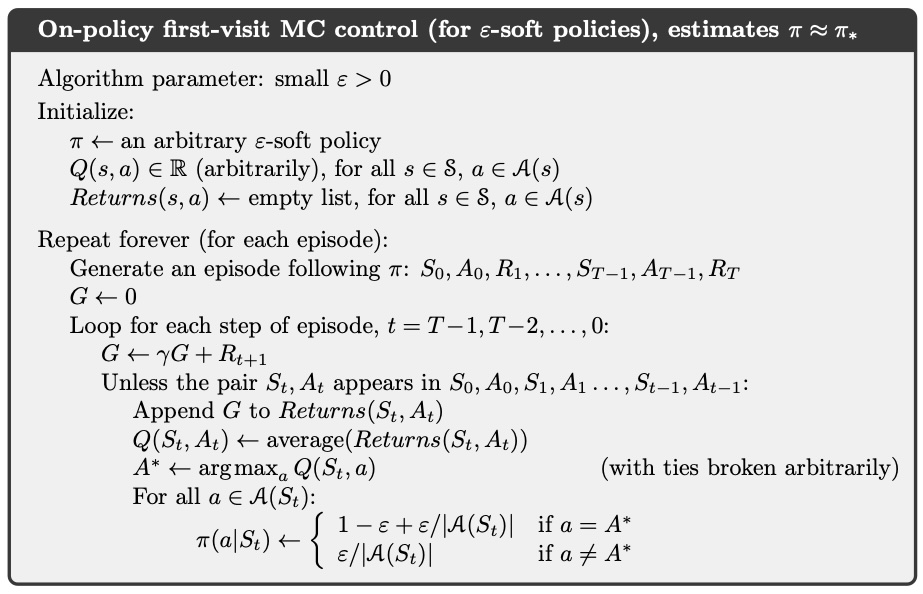
\includegraphics[width=.7\textwidth]{fig/On-policy-first-visit-MC}
	\end{algorithm}
	
	%	\TPMargin{0mm}%
	%	\begin{textblock}{4.3}(10.1, 5.2) \small
		%		\begin{tcolorbox}[colback=blue!5!white]\footnotesize
			%			\hspace{-0.9cm} \faCaretSquareRight ~	\hbox{Los returns se acumulan} \textbf{independientemente} de la política que los observó.
			%			
			%			\hspace{-0.4cm} \faCaretSquareRight	~ No converge a una política subóptima
			%		\end{tcolorbox}
		%	\end{textblock}
	
\end{frame}






%%%%%%%%%%%%%%%%%%%%%%%%%%%%%%%%%%%%%%%%%%%%%%%%%%%%%%%%%%%%%%%%%%%%
%%%%%%%%%%%%%%%%%%%%%%%%%%%%%%%%%%%%%%%%%%%%%%%%%%%%%%%%%%%%%%%%%%%%


\section{Métodos Off-Policy}





%%%%%%%%%%%%%%%%%%%%%%%%%%%%%%%%%%
%%%%%%%%%%%%%%%%%%%%%%%%%%%%%%%%%%
\begin{frame}{Métodos off-Policy}
\scalebox{1.3}{
	\begin{minipage}{.7\textwidth}
	\begin{itemize}
		\item  \key{Métodos off-policy:} Evalúan o mejoran una política diferente a la que se utiliza para generar los datos.
		\item \key{En consecuencia}, dado que los datos provienen de una política diferente, los métodos off-policy generalmente:
		\begin{itemize}
			\item Sufren de mayor varianza.
			\item Son más lentos para converger.
		\end{itemize}
		\item \key{Son más} poderosos y generales.
		\begin{itemize}
			\item Los métodos on-policy son un caso especial.
		\end{itemize}
		\item Pueden aplicarse para \key{aprender a partir de datos generados} por un controlador convencional no basado en aprendizaje, o por un experto humano.
	\end{itemize}

\end{minipage}}
	
\end{frame}







%%%%%%%%%%%%%%%%%%%%%%%%%%%%%%%%%%%%%%%%%%%%%%%%%%%%%%%%%%%%%%%%%%%%
%%%%%%%%%%%%%%%%%%%%%%%%%%%%%%%%%%%%%%%%%%%%%%%%%%%%%%%%%%%%%%%%%%%%

\subsection{Predicción Off-policy MC}


%%%%%%%%%%%%%%%%%%%%%%%%%%%%%%%%%%
%%%%%%%%%%%%%%%%%%%%%%%%%%%%%%%%%%
\begin{frame}{Evaluación de Políticas Monte-Carlo (Off-Policy)}{Muestreo por Importancia}		
	\begin{itemize}
		\item Consideremos el problema de predicción, en el cual tanto la \key{política objetivo} (\textit{$\pi$, target policy}) como la \key{política de comportamiento} (\textit{$b$, behavior policy}) están fijas.
		\begin{itemize}
			\item Queremos estimar \( v_\pi \) o \( q_\pi \), pero solo tenemos episodios generados siguiendo la política \( b \), donde \( b \neq \pi \).
		\end{itemize}
		
		\item \textbf{$b()$ debe cumplir ciertas condiciones.}
		
			\begin{itemize}
				\item \key{Suposición de cobertura:} Toda acción tomada bajo \( \pi \) también debe tomarse, al menos ocasionalmente, bajo \( b \). 
				
						\hfil {\large $\pi(a|s) > 0 \implies b(a|s) > 0.$}
		
				\item \( b() \) debe ser \key{estocástica}.
				
				\hfil A pesar de que $\pi(a|s) = 0$, debe cumplirse $b(a|s) > 0.$
			\end{itemize}
		
		\item Casi todos los métodos \textit{off-policy} utilizan el \key{muestreo de importancia} (esquema general):
		
			\begin{itemize}
				\item Queremos calcular un valor esperado bajo una distribución objetivo \( \pi \):
				$\ds
				\mathbb{E}_\pi[f(x)] = \int f(x) \pi(x) dx,
				$
				
				\item Podemos expresarlo como 
				$\ds
				\mathbb{E}_\pi[f(x)] = \int f(x) \frac{\pi(x)}{b(x)} b(x) dx = \int f(x) w(x) b(x) dx,
				$
				con $\ds w(x) = \frac{\pi(x)}{b(x)}.$
				
				\begin{itemize}
					\item \key{Coeficiente de muestreo de importancia:} $\ds w(x)$
					\item $\ds \mathbb{E}_\pi \big[ f(x) \big] =  \mathbb{E}_{b} \Big[ f(x)\cdot w(x) \Big]$
				\end{itemize}
				
				\item Entonces \fbox{$\ds \mathbb{E}_\pi[f(x)] \approx \frac{1}{N} \sum_{i=1}^N f(x_i) w(x_i)$ tomando muestras $x_i\sim b(x)$}
			\end{itemize}
	\end{itemize}
		
\TPMargin{0mm}%
\begin{textblock}{5}(10.5, 11.3) \small
	
\includegraphics[width=.5\textwidth]{fig/ImportanceSampling}
	\raisebox{5.5\height}{${\color{red} G_\pi(s)}=\color{ForestGreen}w(s) \color{blue}G_b(s)$}
	\end{textblock}


\end{frame}




%%%%%%%%%%%%%%%%%%%%%%%%%%%%%%%%%%
%%%%%%%%%%%%%%%%%%%%%%%%%%%%%%%%%%
\begin{frame}{Adaptación del Muestreo por Importancia para Predicción}		
	\begin{itemize}
		\item \key{Nuestro objetivo} es estimar $v_\pi(s)$ muestreando con una política $b(s)$ y usando muestreo por importancia.
		
		\item Consideramos  un \key{episodio aleatorio:} $H_{S_t}=A_t, S_{t+1}, A_{t+1}, \dots, S_T$
		
		\item \key{Las probabilidades} bajo las políticas $ \pi $ y $ b $ \key{son:}
		
			\begin{itemize}
				\item $ $ \vskip-.7\baselineskip
				
				$\begin{array}{ll}
					P(H_{S_t} \sim \pi) &\ds = P_\pi\{A_t, S_{t+1}, A_{t+1}, \dots, S_T \mid S_t, A_{t:T-1}\} \\
					&\ds= \pi(A_t \mid S_t) p(S_{t+1} \mid S_t, A_t) \pi(A_{t+1} \mid S_{t+1}) \cdots p(S_T \mid S_{T-1}, A_{T-1}) \\
					&\ds= \prod_{k=t}^{T-1} \pi(A_k \mid S_k) p(S_{k+1} \mid S_k, A_k),
				\end{array}$
			
				\item $\ds P(H_{S_t} \sim b) = \prod_{k=t}^{T-1} b(A_k \mid S_k) p(S_{k+1} \mid S_k, A_k)$
			\end{itemize}
			
		\item El \key{peso de importancia} (\textit{importance-sampling ratio}) para un episodio es:
		
		\hfil $ \ds
		w(H_{S_t}) = \rho_{t:T-1} = \prod_{k=t}^{T-1} \frac{\pi(A_k|S_k)}{b(A_k|b_k)}.
		$
		
		\item \textbf{Reescribimos el valor esperado:} $\ds v_\pi(s) = \mathbb{E}_\pi[G_t \mid S_t = s] = \mathbb{E}_b	[\rho_{t:T-1} G_t \mid S_t = s]$
		
	\end{itemize}

\end{frame}



%%%%%%%%%%%%%%%%%%%%%%%%%%%%%%%%%%
%%%%%%%%%%%%%%%%%%%%%%%%%%%%%%%%%%
\begin{frame}{Predicción Off-Policy con Muestreo por Importancia}
\begin{itemize}
	\item Los pasos de tiempo serán \key{consecutivos}. No se ``resetea'' para cada episodio.
	
	\item  \( \mathcal{T}(s) \) es el \key{conjunto de  pasos de tiempo} en los que el estado \( s \) es visitado
		\begin{itemize}
			\item  \textbf{Primera Visita}:  los pasos de tiempo en los que se realizaron las \textit{primeras visitas} a \( s \) dentro de sus episodios
			\item  \textbf{Todas las Visitas}: \textit{todos} los pasos de tiempo donde $s$ fue visitado.
		\end{itemize}

	\item  \( {T}(t) \): el \key{primer tiempo} de terminación posterior al tiempo \( t \).
	
	\item \( G_t \):  el \key{retorno} después de \( t \) hasta \( T(t) \).
	
	\item Luego, \( \{ G_t \}_{t \in \mathcal{T}(s)} \) son los \textbf{retornos relacionados} con el estado \( s \)
	
	\item \( \{ \rho_{t : T(t)-1} \}_{t \in \mathcal{T}(s)} \) son los correspondientes \key{coeficientes de muestreo por importancia}.
	
	\item \key{Muesteo por importancia ordinario:} Para estimar \( v_\pi(s) \), escala los retornos por los coeficientes de muestreo por importancia y promedia los resultados:
	\[
	V(s) = \frac{\sum_{t \in \mathcal{T}(s)} \rho_{t:T(t)-1} G_t}{|\mathcal{T}(s)|}.
	\]
	
	\item \key{ Muestreo de importancia ponderado:}
	\[
	V(s) \stackrel{\cdot}{=} \frac{\sum_{t \in {\cal T}(s)} \rho_{t:T(t)-1} G_t}{\sum_{t \in {\cal T}(s)} \rho_{t:T(t)-1}}, \text{ \color{black} o cero si el denominador es cero. }
	\]
	
	
	
\end{itemize}

\end{frame}



%%%%%%%%%%%%%%%%%%%%%%%%%%%%%%%%%%
%%%%%%%%%%%%%%%%%%%%%%%%%%%%%%%%%%
\begin{frame}{Comparación entre Muestreo de Importancia Ordinario y Ponderado}
	
\noindent\scalebox{0.6}{
~ ~\begin{minipage}{\textwidth}
\begin{tabular}{>{\raggedright\arraybackslash}m{3cm} >{\raggedright\arraybackslash}m{10cm} >{\raggedright\arraybackslash}m{10cm}}
	\toprule
	\textbf{Características} & \textbf{Muestreo de Importancia Ordinario} & \textbf{Muestreo de Importancia Ponderado} \\
	\midrule
	\textbf{Fórmula de Estimación} & 
	\[
	V(s) \stackrel{\cdot}{=} \frac{\sum_{t \in \mathcal{T}(s)} \rho_{t:T(t)-1} G_t}{|\mathcal{T}(s)|}.
	\]
	Promedio simple de retornos escalados por las razones de importancia.
	&
	\[
	V(s) \stackrel{\cdot}{=} \frac{\sum_{t \in \mathcal{T}(s)} \rho_{t:T(t)-1} G_t}{\sum_{t \in \mathcal{T}(s)} \rho_{t:T(t)-1}},
	\]
	% \quad \text{o cero si el denominador es cero.} \quad \text{(5.6)}
	Promedio ponderado de retornos escalados por las razones de importancia.
	\\
		\midrule
	\mc{3}{c}{\bf Primera Visita} \\
	\midrule
	\midrule
	\textbf{Sesgo} & 
	\begin{itemize}
		\item \textbf{No sesgado}: $\mathbb{E}[V(s)] = v_\pi(s)$.
	\end{itemize}
	&
	\begin{itemize}
		\item \textbf{Sesgado}: $\mathbb{E}[V(s)] \approx v_b(s)$.
		\item El sesgo converge a cero asintóticamente.
	\end{itemize}
	\\
	\midrule
	\textbf{Varianza} & 
	\begin{itemize}
		\item \textbf{Alta y potencialmente ilimitada}: Depende de la variabilidad de las razones $\rho$.
		\item Puede ser extrema si $\rho$ es grande (e.g., transparencia posterior).
	\end{itemize}
	&
	\begin{itemize}
		\item \textbf{Menor varianza}: Normalización reduce el impacto de $\rho$ grandes.
		\item La varianza converge a cero si los retornos están acotados, incluso si $\text{Var}(\rho)$ es infinita.
	\end{itemize}
	\\
	\midrule
	\textbf{Convergencia} & 
	\begin{itemize}
		\item La expectativa está alineada con $v^\pi(s)$, pero con alta varianza puede requerir más muestras.
	\end{itemize}
	&
	\begin{itemize}
		\item Aunque sesgado, la menor varianza suele conducir a estimaciones más estables y eficientes en la práctica.
	\end{itemize}
	\\
	\midrule
	\textbf{Preferencia Práctica} & 
	\begin{itemize}
		\item Menos preferido debido a la alta varianza.
		\item Más fácil de extender a métodos aproximados usando aproximación funcional.
	\end{itemize}
	&
	\begin{itemize}
		\item Generalmente preferido en la práctica por su varianza significativamente menor.
		\item Usado comúnmente en algoritmos de Monte Carlo de todas las visitas.
	\end{itemize}
	\\
	\midrule \midrule \midrule
	\textbf{Todas las Visitas} & 
	\begin{itemize}
		\item Ambas variantes (ordinario y ponderado) son sesgadas en métodos de visita múltiple.
		\item El sesgo disminuye asintóticamente con el aumento del número de muestras.
	\end{itemize}
	&
	Son preferidos "Todas las visitas" porque
	\begin{itemize}
		\item Eliminan la necesidad de llevar un registro de qué estados han sido visitados 
		\item Son mucho más fáciles de extender a aproximaciones.
	\end{itemize}
	\\
	\bottomrule
\end{tabular}
\end{minipage}}

\end{frame}




%%%%%%%%%%%%%%%%%%%%%%%%%%%%%%%%%%
%%%%%%%%%%%%%%%%%%%%%%%%%%%%%%%%%%
%%%%%%%%%%%%%%%%%%%%%%%%%%%%%%%%%%
%%%%%%%%%%%%%%%%%%%%%%%%%%%%%%%%%%
\begin{frame}{Estimación off-policy del valor de un estado en Blackjack}{Curvas de aprendizaje}
	\begin{itemize}
		\item Se aplicaron tanto métodos de \textbf{muestreo de importancia ordinario} como \textbf{muestreo de importancia ponderado} para estimar el valor de un único estado en Blackjack.
		\item Estado evaluado: \(v_\pi(s) \approx 0.27726\) para 100 millones de episodios on-policy
			\begin{itemize}
				\item $s=$\textit{(El crupier muestra un dos,
			 La suma de las cartas del jugador es 13,
			 El jugador tiene un as utilizable)}
				
				\end{itemize}
						
		\item La \textbf{política de comportamiento} es pedir o plantarse con igual probabilidad.
		\item La \textbf{política objetivo} consiste en plantarse solo con una suma de 20 o 21.
	\end{itemize}
	

	\noindent 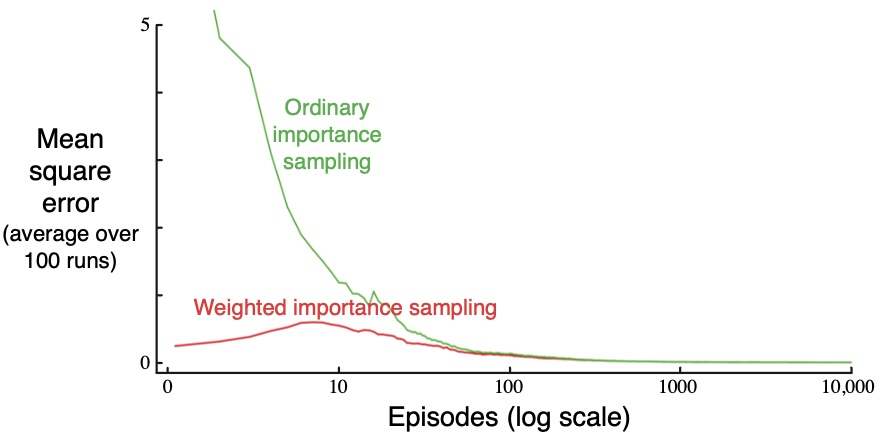
\includegraphics[width=.7\textwidth]{fig/WeightedImportanceSampling}

	
\TPMargin{0mm}%
\begin{textblock}{7}(8, 8) \small
	$
	\text{ECM} = \frac{1}{N} \sum_{i=1}^N \left( \hat{v}^{(i)}(s) - v_\pi(s) \right)^2
	$
	Donde:
	\begin{itemize}
		\item \(N = 100\): Número de ejecuciones independientes.
		\item \(\hat{v}^{(i)}(s)\): Estimación en la \(i\)-ésima ejecución.
		\item \(v_\pi(s) = 0.27726\): Valor verdadero del estado.
		\item[]
		\item Convergen al valor verdadero después de \textbf{10,000 episodios}.
	\end{itemize}
	%\raisebox{5.5\height}{${\color{red} G_\pi(s)}=\color{ForestGreen}w(s) \color{blue}G_b(s)$}
\end{textblock}

\end{frame}



%%%%%%%%%%%%%%%%%%%%%%%%%%%%%%%%%%
%%%%%%%%%%%%%%%%%%%%%%%%%%%%%%%%%%


\begin{frame}{Varianza Infinita en Muestreo de Importancia Ordinario}
\begin{itemize}
	\item Las estimaciones del muestreo de importancia ordinario típicamente tienen \textbf{varianza infinita} si los retornos escalados tienen varianza infinita.
		\begin{itemize}
			\item Esto es común en aprendizaje \textit{off-policy} si las trayectorias contienen bucles.
		\end{itemize}
	\item Ejemplo:

	~ \hspace{-4em} 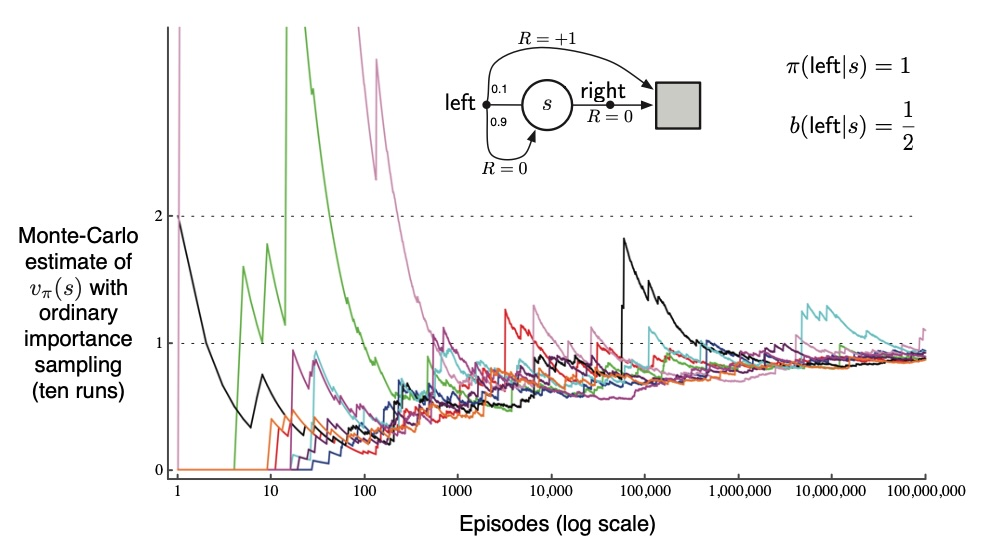
\includegraphics[width=0.6\textwidth]{fig/OrdinaryImportanceSampling}
	
	\begin{itemize}
	\item El algoritmo de \key{muestreo de importancia ponderado} \textbf{resuelve este problema}:
	\begin{itemize}
		\item Estimación de \(V(s)\) es exactamente 1 después del primer episodio consistente.
		\item Los retornos inconsistentes (terminados con derecha) tienen una razón de muestreo de importancia de \(\rho = 0\) y no contribuyen al cálculo.
	\end{itemize}
	\end{itemize}
	
\end{itemize}

\TPMargin{0mm}%
\begin{textblock}{8.5}(7.7, 4.7) 
\scalebox{.8}{
\begin{minipage}{\textwidth}
	\begin{itemize}
		\item[]~
		\begin{itemize}
		\item $\ds v_\pi(s) = \mathbb{E}_\pi[G_t \mid S_t = s] = \mathbb{E}_b	[\rho_{t:T-1} G_t \mid S_t = s]$
		\item $\text{Var}[X] = \mathbb{E}\left[(X - \bar{X})^2\right] = \mathbb{E}[X^2] - \bar{X}^2.$
		\item $\mathbb{E}_b\left[\left( \prod_{t=0}^{T-1} \frac{\pi(A_t \mid S_t)}{b(A_t \mid S_t)} G_0 \right)^2\right]=$ \footnotesize
		\begin{align*}
			= & \; \frac{1}{2} \cdot 0.1 \left( \frac{1}{0.5} \right)^2 
			\quad \text{(el episodio de longitud 1)} \\
			& + \frac{1}{2} \cdot 0.9 \cdot \frac{1}{2} \cdot 0.1 \left( \frac{1}{0.5 \cdot 0.5} \right)^2 
			\quad \text{(el episodio de longitud 2)} \\
			& + \frac{1}{2} \cdot 0.9 \cdot \frac{1}{2} \cdot 0.9 \cdot \frac{1}{2} \cdot 0.1 \left( \frac{1}{0.5 \cdot 0.5 \cdot 0.5} \right)^2 
			\quad \text{(el episodio de longitud 3)} \\
			& + \cdots \\ 
			= & \;  0.1  \sum_{k=1}^\infty \left(\frac{1}{2}\right)^k 0.9^{k-1}  2^{2k} = 0.1 \sum_{k=0}^\infty 0.9^k \cdot 2^k \cdot 2 = 0.2 \sum_{k=0}^\infty 1.8^k = \infty. 
		\end{align*}
		
		\vskip-0.5cm $ $
		\item Existe \key[red]{desalineación de políticas}: $b()<<\pi()$.
		
		\end{itemize}
	\end{itemize}
\end{minipage}
}
	
	
\end{textblock}

\end{frame}



%%%%%%%%%%%%%%%%%%%%%%%%%%%%%%%%%%
%%%%%%%%%%%%%%%%%%%%%%%%%%%%%%%%%%

\begin{frame}{Versión Incremental}
	\begin{itemize}
		\item Estamos interesados en $\ds V(s)=\mathbb{E}_\pi[G_t|S_t=s]$ y tenemos una secuencia de retornos \(G_1, G_2, \ldots, G_{n-1}\), todos comenzando en el mismo estado $s$.
		
		\item Generamos un episodio desde $s$, calculamos $G_n$ y actualizamos $V_{n+1}$ para todo $n\geq 1$.

		\item \key{On-policy:} $\ds V(s)  =\mathbb{E}_\pi[G_t|S_t=s] \approx V_n=\frac{\sum_{k=1}^{n-1} G_k}{n-1}$.
		\begin{enumerate}
			\item $V_{n+1}= V_n + \frac{1}{n} \left(G_{n} - V_n\right)$.
		\end{enumerate}
		
		
		\item \key{Off-policy ordinario:} $\ds V(s) = \mathbb{E}_b	[{\color{red} \rho_{t:T-1}} G_t \mid S_t = s] \approx  V_n=\frac{\sum_{k=1}^{n-1} {\color{red} \rho_{t_k:T(t_k)-1}} G_k}{n-1} =  \frac{\sum_{k=1}^{n-1} {\color{red} W_k} G_k}{n-1}$. 
		
		\begin{enumerate}
			\item \(W_{n} = {\large\rho}_{t_{n}:T(t_{n})-1}\) 
			\item $V_{n+1}=V_n + \frac{1}{n} \left( {\color{red} W_{n}} G_{n} - V_n \right )$
		\end{enumerate}
		
		\item  \key{Off-policy ponderado:}
		$\ds V(s) =  \mathbb{E}_b	[\rho_{t:T-1} G_t \mid S_t = s] \approx V_n=\frac{\sum_{k=1}^{n-1} {\color{red} \rho_{t_k:T(t_k)-1}}  G_k}{\color{orange} \sum_{k=1}^{n-1} \rho_{t_k:T(t_k)-1}} =  \frac{\sum_{k=1}^{n-1} {\color{red} W_k} G_k}{\color{orange} \sum_{k=1}^{n-1} W_k}$.
		
		\begin{enumerate}
			\item \( {\color{red}W_{n}} = {\large\rho}_{t_{n}:T(t_{n})-1}\) 
			\item ${\color{orange} C_{n}} = C_{n-1} + W_{n}$
			\item $\ds V_{n+1}=V_n + {\color{orange} \frac{{\color{red} W_{n}}}{C_{n}} } \left(  G_{n} - V_n \right )$
		\end{enumerate}
	\end{itemize} 

\end{frame}









%%%%%%%%%%%%%%%%%%%%%%%%%%%%%%%%%%
%%%%%%%%%%%%%%%%%%%%%%%%%%%%%%%%%%
\begin{frame}{Predicción  \textit{Off-policy} MC todas las visitas para estimar $V \approx v_\pi$}

\begin{algorithm}[H]
	\caption{Predicción fuera de política MC para estimar \(V\approx v_\pi\)}
	\label{alg:off_policy_mc}
	\begin{algorithmic} 	\small
		\REQUIRE una política objetivo arbitraria \(\pi\)
		\STATE INICIALIZAR, para todos los \(s \in S\):
		\STATE \hspace{1em} \(V(s) \in \mathbb{R}\) (inicializado arbitrariamente)
		\STATE \hspace{1em} \(C(s) \gets 0\) (pesos acumulativos de muestreo de importancia)
		\WHILE{True, (para cada episodio)}
		\STATE SELECCIONAR una política de comportamiento \(b\) con cobertura de \(\pi\)
		\STATE GENERAR un episodio siguiendo \(b\): \(S_0, A_0, R_1, S_1, \dots, S_{T-1}, A_{T-1}, R_T\)
		\STATE \(G \gets 0\) \COMMENT{Inicializar el retorno acumulado}
		\STATE \(W \gets 1\) \COMMENT{Inicializar el peso acumulado}
		\FOR {cada paso del episodio en orden inverso \(t = T-1, T-2, \dots, 0\), mientras \(W \neq 0\):}
		\STATE \(G \gets \gamma G + R_{t+1}\) \qquad \qquad \qquad \quad  \COMMENT{Actualizar el retorno acumulado}
		\STATE \(C(S_t) \gets C(S_t) + W\) \qquad \qquad \qquad  \COMMENT{Actualizar el peso acumulado para \(S_t\)}
		\STATE \(V(S_t) \gets V(S_t) + \frac{W}{C(S_t)} [G - V(S_t)]\) \COMMENT{Actualización incremental del valor del estado \(S_t\)}
		\STATE \(\ds W \gets W \cdot \frac{\pi(A_t|S_t)}{b(A_t|S_t)}\) \qquad \qquad \qquad \COMMENT{Actualizar el peso de importancia}
		\ENDFOR
		\ENDWHILE
	\end{algorithmic}
\end{algorithm}

\TPMargin{0mm}%
\begin{textblock}{5}(10.7, 4.7) 
	\begin{tcolorbox}[colback=red!2!white]
	 \hspace*{-0.5cm}\parbox{5cm}{	
	 	\begin{enumerate}
			\item \(W_{n} = {\large\rho}_{t_{n}:T(t_{n})-1}\) 
			\item ${\color{orange} C_{n}} = C_{n-1} + W_{n}$
			\item $\ds V_{n+1}=V_n + {\color{orange} \frac{W_{n}}{C_{n}} } \left(  G_{n} - V_n \right )$
		\end{enumerate}}
	\end{tcolorbox}
\end{textblock}

\end{frame}


%%%%%%%%%%%%%%%%%%%%%%%%%%%%%%%%%%
%%%%%%%%%%%%%%%%%%%%%%%%%%%%%%%%%%
\begin{frame}{Predicción  \textit{Off-policy} MC todas las visitas para estimar $Q \approx q_\pi$}{\cite{Sutton2018}}	
	\begin{algorithm}[H]
		\caption{Predicción MC off-Policy, para estimar \(Q \approx q_\pi\)}
		
		\centering 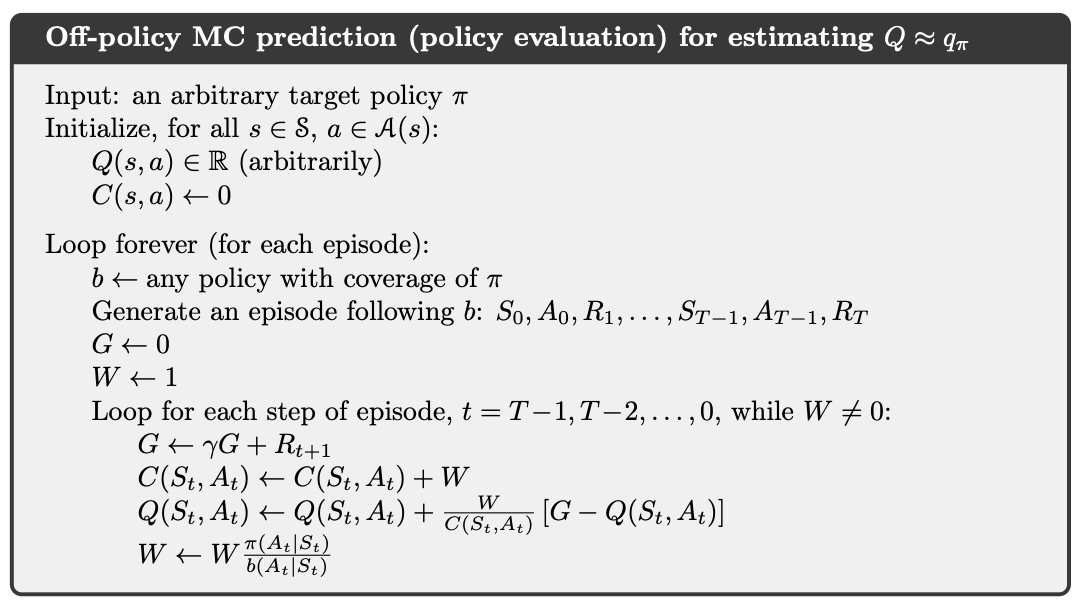
\includegraphics[width=.8\textwidth]{fig/off-policy-MC-prediction}
	\end{algorithm}
	
\end{frame}

%%%%%%%%%%%%%%%%%%%%%%%%%%%%%%%%%
%%%%%%%%%%%%%%%%%%%%%%%%%%%%%%%%%%




%%%%%%%%%%%%%%%%%%%%%%%%%%%%%%%%%%
%%%%%%%%%%%%%%%%%%%%%%%%%%%%%%%%%%

\subsection{Control Off-policy}



%%%%%%%%%%%%%%%%%%%%%%%%%%%%%%%%%%
%%%%%%%%%%%%%%%%%%%%%%%%%%%%%%%%%%
\begin{frame}{Control Monte Carlo Off-Policy}
\begin{itemize}
	\item Los métodos de control Monte Carlo \textbf{off-policy} \key{se caracterizan} porque
		\begin{itemize}
			\item Siguen una \textbf{política de comportamiento} para aprender (experiencia, episodios), $b(a|s)$.
			\item Mejoran una \textbf{política objetivo}, $\pi(a|s)$.
		\end{itemize} 
	
	\item \key{Condiciones} sobre la política de comportamiento $b()$:
		\begin{itemize}
			\item Política de \textbf{comportamiento suave} (\textit{soft}). $b(a|s)>0$ $\forall a$
				\begin{itemize}
				\item \textbf{Cobertura}. Si $\pi(a|s)>0$,  $b(a|s)>0$.	
				\item \textbf{Estocástica}. Si $\pi(a|s)=0$,  $b(a|s)>0$.
				\end{itemize}
			\item P.e. que sea \textbf{$\epsilon$-soft}: \(\ds b(a|s) \geq \frac{\epsilon}{|\mathcal{A}(s)|}\) para todos los \(s \in \mathcal{S}\) y \(a \in \mathcal{A}\), donde \(\epsilon > 0\).
		\end{itemize}
		
	\item Nos basamos en el \key{Método de Iteración de Políticas General}:
	
	
\begin{columns}
	\begin{column}{.6\textwidth}
		\begin{itemize}
			\item \key{Evaluación}
				\begin{itemize}
					\item $b()$ será  una política soft
					\item Aplicar Predicción MC off-policy para estimar $Q\approx q_\pi$
				\end{itemize}
				
			\item \key{Mejora}
				\begin{itemize}
					\item Aplicar una política greedy sobre $Q$
				\end{itemize}
		\end{itemize}
	\end{column}
		\begin{column}{.2\textwidth}
		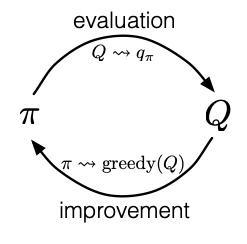
\includegraphics[width=\textwidth]{fig/MejoraPolitica}
	\end{column}
\end{columns}	
	
\end{itemize}
\end{frame}








%%%%%%%%%%%%%%%%%%%%%%%%%%%%%%%%%%
%%%%%%%%%%%%%%%%%%%%%%%%%%%%%%%%%%
\begin{frame}{Control Monte Carlo sin Inicios Exploratorios}
	

\begin{algorithm}[H]
	\caption{\textit{Off-policy} MC control  para estimar $\pi \approx \pi_*$}

\centering	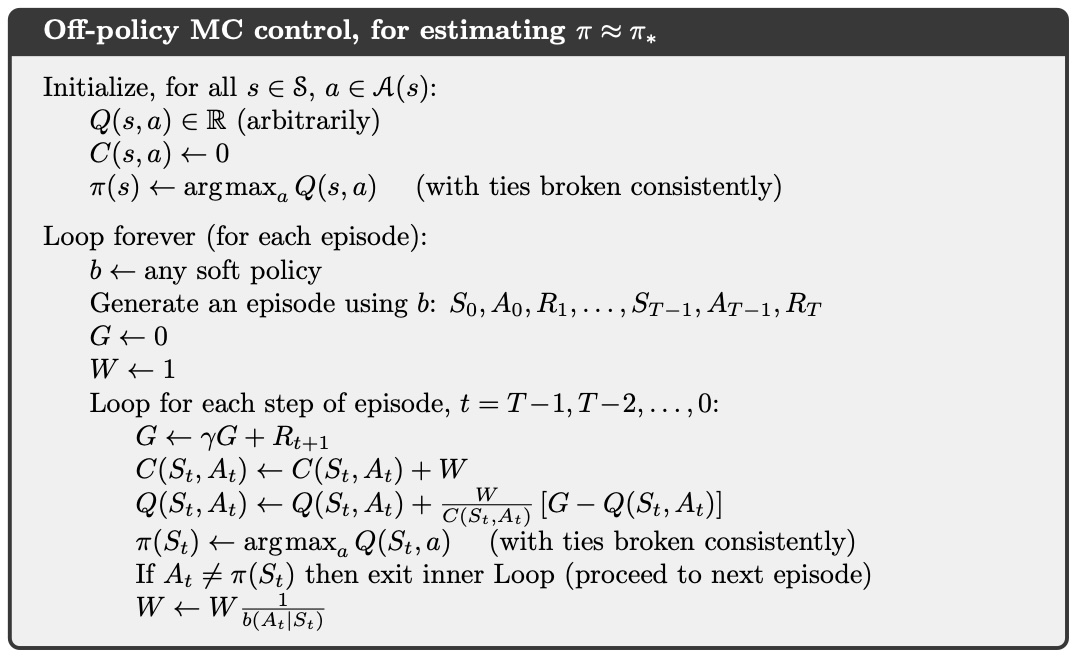
\includegraphics[width=.8\textwidth]{fig/off-policy-MC-control}
\end{algorithm}

\end{frame}





%%%%%%%%%%%%%%%%%%%%%%%%%%%%%%%%%%
%%%%%%%%%%%%%%%%%%%%%%%%%%%%%%%%%%
% BIBLIOGRAFÍA
%%%%%%%%%%%%%%%%%%%%%%%%%%%%%%%%%%
%%%%%%%%%%%%%%%%%%%%%%%%%%%%%%%%%%


%%%%%%%%%%%%%%%%%%%%%%%%%%%%%%%%%%%%%%%%%%%%%%%%%%%%%%%%%%%%%%%%%%%%
%%%%%%%%%%%%%%%%%%%%%%%%%%%%%%%%%%%%%%%%%%%%%%%%%%%%%%%%%%%%%%%%%%%%

\section{Referencias}



% Redefinimos la apariencia
%\setbeamertemplate{headline}{}
%\setbeamertemplate{frametitle}{\vskip 0.5cm	\small{\textbf{\insertframetitle}}}
%\setbeamertemplate{footline}{}




% Mostramos la bibliografía
% \begin{frame}[allowframebreaks] %% Si ocupa más de una página
%\begin{frame}[allowframebreaks]{Referencias -} %% Si hay sólo una página

\begin{frame}{Referencias} %% Si hay sólo una página
\nocite{Sutton2018, silver2015, Hado2018Lecture3}

	% \vskip -5cm %% Para ajustar la distancia al comienzo	
	%\bibliography{references}	
	\printbibliography[heading=none]
\end{frame}    


		
%%%%%%%%%%%%%%%%%%%%%%%%%%%%%%%%%%
%%%%%%%%%%%%%%%%%%%%%%%%%%%%%%%%%%

\end{document}

%%%%%%%%%%%%%%%%%%%%%%%%%%%%%%%%%%
%%%%%%%%%%%%%%%%%%%%%%%%%%%%%%%%%%


\end{document}



